%This is a Tex Version of NE 806 Homework Template
%
\documentclass{amsart}
\setlength{\textheight}{9in}
\setlength{\topmargin}{-0.25in}
\setlength{\textwidth}{7in}
\setlength{\evensidemargin}{-0.25in}
\setlength{\oddsidemargin}{-0.25in}
\usepackage{amsfonts}
\usepackage[utf8]{inputenc}
\usepackage[T1]{fontenc}
\usepackage{graphicx} 
\usepackage[export]{adjustbox}
% needed to include these graphics
%\graphicspath{{./Pictures/}}      % only in case you want to keep the pictures in a separate
                                  % subdirectory; also see the appropriate line below
\usepackage{caption}
\usepackage{subcaption}
\usepackage{float}
\usepackage{framed}
\newcounter{temp}
\theoremstyle{definition}
\newtheorem{Thm}{Theorem}
\newtheorem{Prob}{Problem}
\newtheorem*{Def}{Definition}
\newtheorem*{Ans}{Answer}
\newcommand{\dis}{\displaystyle}
\newcommand{\dlim}{\dis\lim}
\newcommand{\dsum}{\dis\sum}
\newcommand{\dint}{\dis\int}
\newcommand{\ddint}{\dint\!\!\dint}
\newcommand{\dddint}{\dint\!\!\dint\!\!\dint}
\newcommand{\dt}{\text{d}t}
\newcommand{\dA}{\text{d}A}
\newcommand{\dV}{\text{d}V}
\newcommand{\dx}{\text{d}x}
\newcommand{\dy}{\text{d}y}
\newcommand{\dz}{\text{d}z}
\newcommand{\dw}{\text{d}w}
\newcommand{\du}{\text{d}u}
\newcommand{\dv}{\text{d}v}
\newcommand{\ds}{\text{d}s}
\newcommand{\dr}{\text{d}r}
\newcommand{\dth}{\text{d}\theta}
\newcommand{\bbR}{\mathbb{R}}
\newcommand{\bbN}{\mathbb{N}}
\newcommand{\bbQ}{\mathbb{Q}}
\newcommand{\bbZ}{\mathbb{Z}}
\newcommand{\bbC}{\mathbb{C}}
\newcommand{\dd}[2]{\dfrac{\text{d}#1}{\text{d}#2}}
\newcommand{\dydx}{\dfrac{\text{d}y}{\text{d}x}}
\renewcommand{\labelenumi}{{\normalfont \arabic{enumi}.}}
\renewcommand{\labelenumii}{{\normalfont \alph{enumii}.}}
\renewcommand{\labelenumiii}{{\normalfont \roman{enumiii}.}}
\font \bggbf cmbx18 scaled \magstep2
\font \bgbf cmbx10 scaled \magstep2
\usepackage{fancyhdr}
\usepackage{lipsum}
\usepackage{amsmath}
\usepackage{empheq}
\newcommand*\widefbox[1]{\fbox{\hspace{2em}#1\hspace{2em}}}
% Clear the header and footer
\fancyhead{}
\fancyfoot{}
% Set the right side of the footer to be the page number
\rfoot{\thepage}
\fancyhf{}
\pagestyle{fancy}
\begin{document}
\LARGE{NE-806: Neutronics}
 
\large
Homework \#4 due Thurs. November 15th, 2018
 
Solutions by: Daniel M Nichols
\newline
\bigskip
%%%%%%%%%%%%%%%%%%%%%%%%%%%%%%%%%%%%%%%%%%%%%%%%%%%%%%%%%%%%%%%%%%%%%%%%%%%%%%%%%%%%%%%%%%%%%%%%%%%%%%%%%%%%%%%%%%%%%%%%%%%
\textbf{Problem 1:} \newline For the following one-speed diffusion problems write: (1) the appropriate from of the diffusion equation (with a sketch showing the problem geometry), (2) the form of the most general solution (including any particular solution), (3) the boundary/source conditions you would use to find values for any arbitrary constants in your general solution, and (4) an explicit expression for the flux density. Assume a vacuum surrounds the media.
\bigbreak
(a) An infinite homogeneous slab of thickness $T$ has a volumetrically distributed source with a strength $S(x)$ = $S_0x^2$ neutrons $cm^3$ $s^{-1}$ where $x$ is measured from the left surface of the slab.\newline
\bigbreak
(b) An infinite homogeneous cylinder of diameter $T$ contains a uniformly distributed source of strength $S_0$ neutrons $cm^{-3}$ $s^{-1}$.\newline
\bigbreak
(c) A homogeneous sphere of diameter $T$ contains a uniformly distributed source of strength $S_0$ neutrons $cm^{-3}$ $s^{-1}$.\newline
\bigbreak
(d) Two infinite homogeneous slabs each of thickness $T$ are placed a distance $T$ apart. The left slab has a distributed source $S(x)$ = $S_0\cos \alpha x$ neutrons $cm^{-3}$ $s^{-1}$ where $x$ is measured from the outer surface. The outer surface of the other slab is illuminated uniformly by a perpendicular neutron beam of strength $I_0$ neutrons $cm^{-2}$ $s^{-1}$.\newline
\bigbreak
%%%%%%%%%%%%%%%%%%%%%%%%%%%%%%%%%%%%%%%%%%%%%%%%%%%%%%%%%%%%%%%%%%%%%%%%%%%%%%%%%%%%%%%%%%%%%%%%%%%%%%%%%%%%%%%%%%%%%%%%%%%
\newpage
\textbf{Solution}
\bigbreak
a) The approximate form of the diffusion equation for a infinite slab reactor is given below:
\bigbreak
\begin{equation*}
    \frac{d^2}{dx^2}\phi(x) + B^2\phi(x) + \frac{S(x)}{D} = 0
\end{equation*}
 
\begin{figure}[h!]
                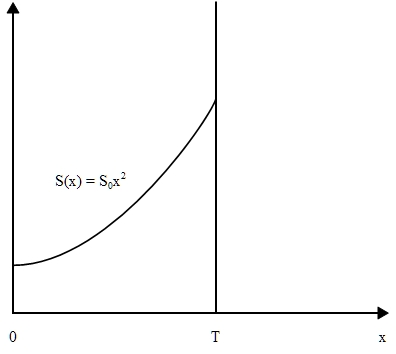
\includegraphics[width=.45\linewidth]{P1a.jpg}
\end{figure}
\bigbreak
The general solution form is shown below:
\bigbreak
\[   \phi(x) = \left\{
\begin{array}{ll}
      Ae^{-Bx} + Ce^{Bx} &  \\
      A'\sinh(Bx) + C'\cosh(Bx) &  \\
\end{array}
\right. , \quad B^2 < 0\]
\bigbreak
\[   \phi(x) = \left\{
\begin{array}{ll}
      Ae^{-iBx} + Ce^{iBx} &  \\
      A'\sin(Bx) + C'\cos(Bx) &  \\
\end{array}
\right. , \quad B^2 > 0\]
\bigbreak
The boundary conditions for this geometry are given below:
\begin{itemize}
    \item $J^+$(0) = 0
    \item $J^-$(T) = 0
\end{itemize}
\bigbreak
Given the general solution above, the homogeneous solution is determined as:
\begin{equation*}
    \phi_h(x) = Ae^{-Bx} + Ce^{Bx}
\end{equation*}
The particular solution is determined to be:
\begin{equation*}
    \phi_p(x) = \frac{2\frac{S_0}{D}}{(B^2)^2} + \frac{\frac{S_0}{D}x^2}{B^2}
\end{equation*}
Using boundary condition 1 and the formula taken from pg 146 of "Nuclear Reactor Physics" by E. E. Lewis:
\begin{equation*}
    J^\mp(x) = \frac{\phi(x)}{4} \pm \frac{D}{2} \phi'(x)
\end{equation*}
An equation relating coefficient $A$ to coefficient $C$, can be determined:
\begin{align*}
    0 &= J^+(0) = \frac{\phi(0)}{4} - \frac{D}{2} \phi'(0) \\
     0 &= 0.25\bigg[\frac{2\frac{S_0}{D}}{(B^2)^2}+A+C\bigg] - \frac{D}{2}\bigg[AB-CB\bigg] \\
     0 &= \bigg[\frac{2\frac{S_0}{D}}{(B^2)^2}+A+C\bigg] - 2D\bigg[AB-CB\bigg] \\
     0 &= A[1-2DB] + C[1+2DB]+\frac{2\frac{S_0}{D}}{(B^2)^2} \\
     A[2DB-1] &= C[1+2DB]+\frac{2\frac{S_0}{D}}{(B^2)^2} \\
     A &= \frac{-C(1+2DB)-\frac{2\frac{S_0}{D}}{(B^2)^2}}{1-2DB}
\end{align*}
Using boundary condition 2:
\begin{align*}
     0 &= J^-(T) = \frac{\phi(T)}{4} + \frac{D}{2} \phi'(T) \\
     0 &= \bigg[\frac{2\frac{S_0}{D}}{(B^2)^2} + \frac{\frac{S_0}{D}T^2}{B^2}+\frac{4DT\frac{S_0}{D}}{B^2}\bigg] + A(e^{BT})[1+2DB]+C(e^{-BT})[1-2DB]
\end{align*}
Substituting in for A:
\begin{align*}
    0 &= \bigg[\frac{2\frac{S_0}{D}}{(B^2)^2} + \frac{\frac{S_0}{D}T^2}{B^2}+\frac{4DT\frac{S_0}{D}}{B^2}\bigg] + \frac{-C(1+2DB)-\frac{2\frac{S_0}{D}}{(B^2)^2}}{1-2DB}(e^{BT})[1+2DB]+C(e^{-BT})[1-2DB] \\
    0 &= C\bigg[(e^{-BT})[1-2DB] - \frac{1+2DB}{1-2DB}(e^{BT})[1+2DB]\bigg] +\bigg[\frac{2\frac{S_0}{D}}{(B^2)^2} + \frac{\frac{S_0}{D}T^2}{B^2}+\frac{4DT\frac{S_0}{D}}{B^2} - \frac{\frac{2\frac{S_0}{D}}{(B^2)^2}}{1-2DB}\bigg] \\
    C &= \frac{\bigg[\frac{\frac{2\frac{S_0}{D}}{(B^2)^2}(e^{BT})[1+2DB]}{1-2DB} - \frac{2\frac{S_0}{D}}{(B^2)^2} - \frac{\frac{S_0}{D}T^2}{B^2}-\frac{4DT\frac{S_0}{D}}{B^2} \bigg]}{\bigg[(e^{-BT})[1-2DB] - \frac{1+2DB}{1-2DB}(e^{BT})[1+2DB]\bigg]}
\end{align*}
Thus the coefficient $A$ is:
\begin{equation*}
    A = \frac{-\frac{\bigg[\frac{\frac{2\frac{S_0}{D}}{(B^2)^2}(e^{BT})[1+2DB]}{1-2DB} - \frac{2\frac{S_0}{D}}{(B^2)^2} - \frac{\frac{S_0}{D}T^2}{B^2}-\frac{4DT\frac{S_0}{D}}{B^2} \bigg]}{\bigg[(e^{-BT})[1-2DB] - \frac{1+2DB}{1-2DB}(e^{BT})[1+2DB]\bigg]}(1+2DB)-\frac{2\frac{S_0}{D}}{(B^2)^2}}{1-2DB}
\end{equation*}
Finally, the explicit formula for the flux in the slab can be solved:
\begin{empheq}[box=\widefbox]{align*}
    \phi(x) &= \frac{-\frac{\bigg[\frac{\frac{2\frac{S_0}{D}}{(B^2)^2}(e^{BT})[1+2DB]}{1-2DB} - \frac{2\frac{S_0}{D}}{(B^2)^2} - \frac{\frac{S_0}{D}T^2}{B^2}-\frac{4DT\frac{S_0}{D}}{B^2} \bigg]}{\bigg[(e^{-BT})[1-2DB] - \frac{1+2DB}{1-2DB}(e^{BT})[1+2DB]\bigg]}(1+2DB)-\frac{2\frac{S_0}{D}}{(B^2)^2}}{1-2DB}e^{-Bx} \\ &+ \frac{\bigg[\frac{\frac{2\frac{S_0}{D}}{(B^2)^2}(e^{BT})[1+2DB]}{1-2DB} - \frac{2\frac{S_0}{D}}{(B^2)^2} - \frac{\frac{S_0}{D}T^2}{B^2}-\frac{4DT\frac{S_0}{D}}{B^2} \bigg]}{\bigg[(e^{-BT})[1-2DB] - \frac{1+2DB}{1-2DB}(e^{BT})[1+2DB]\bigg]}e^{Bx} +\frac{2\frac{S_0}{D}}{(B^2)^2} + \frac{\frac{S_0}{D}x^2}{B^2}
\end{empheq}
 
%###############################################################################
\newpage
\bigbreak
b) The approximate form of the diffusion equation for a infinite cylinder reactor is given below:
\bigbreak
\begin{equation*}
    \frac{d^2}{dr^2}\phi(r) + \frac{1}{r}\frac{d}{dr}\phi(r) +B^2\phi(r) + \frac{S(r)}{D} = 0
\end{equation*}
\begin{figure}[h!]
                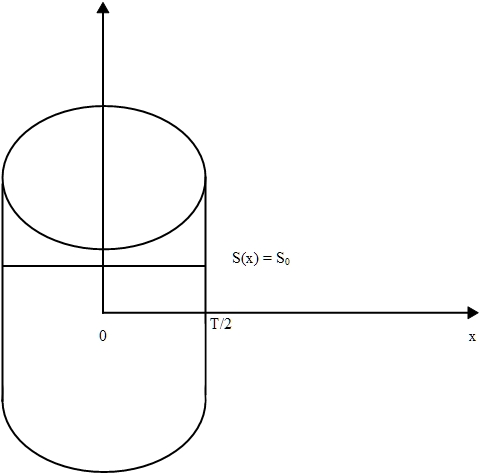
\includegraphics[width=.45\linewidth]{P1b.jpg}
\end{figure}
\bigbreak
The general solution form is shown below:
\bigbreak
\[   \phi(r) = \left\{
\begin{array}{ll}
      AI_0(Br) + CK_0(Br), &  B^2 < 0\\
      AJ_0(Br) + CY_0(Br), &  B^2 > 0\\
\end{array}
\right. \]
\bigbreak
The boundary conditions for this geometry are given below:
\begin{itemize}
    \item $\phi(0) \neq \infty$
    \item $J^-$(T/2) = $J^+$(-T/2) = 0
    \item $\lim_{x\to\infty} \phi(x)$ = 0
\end{itemize}
\newpage
Using boundary condition 1 and the below figure:
\begin{equation*}
    \phi(0) \neq \infty, \quad so \quad C = 0
\end{equation*}
\begin{figure}[h!]
                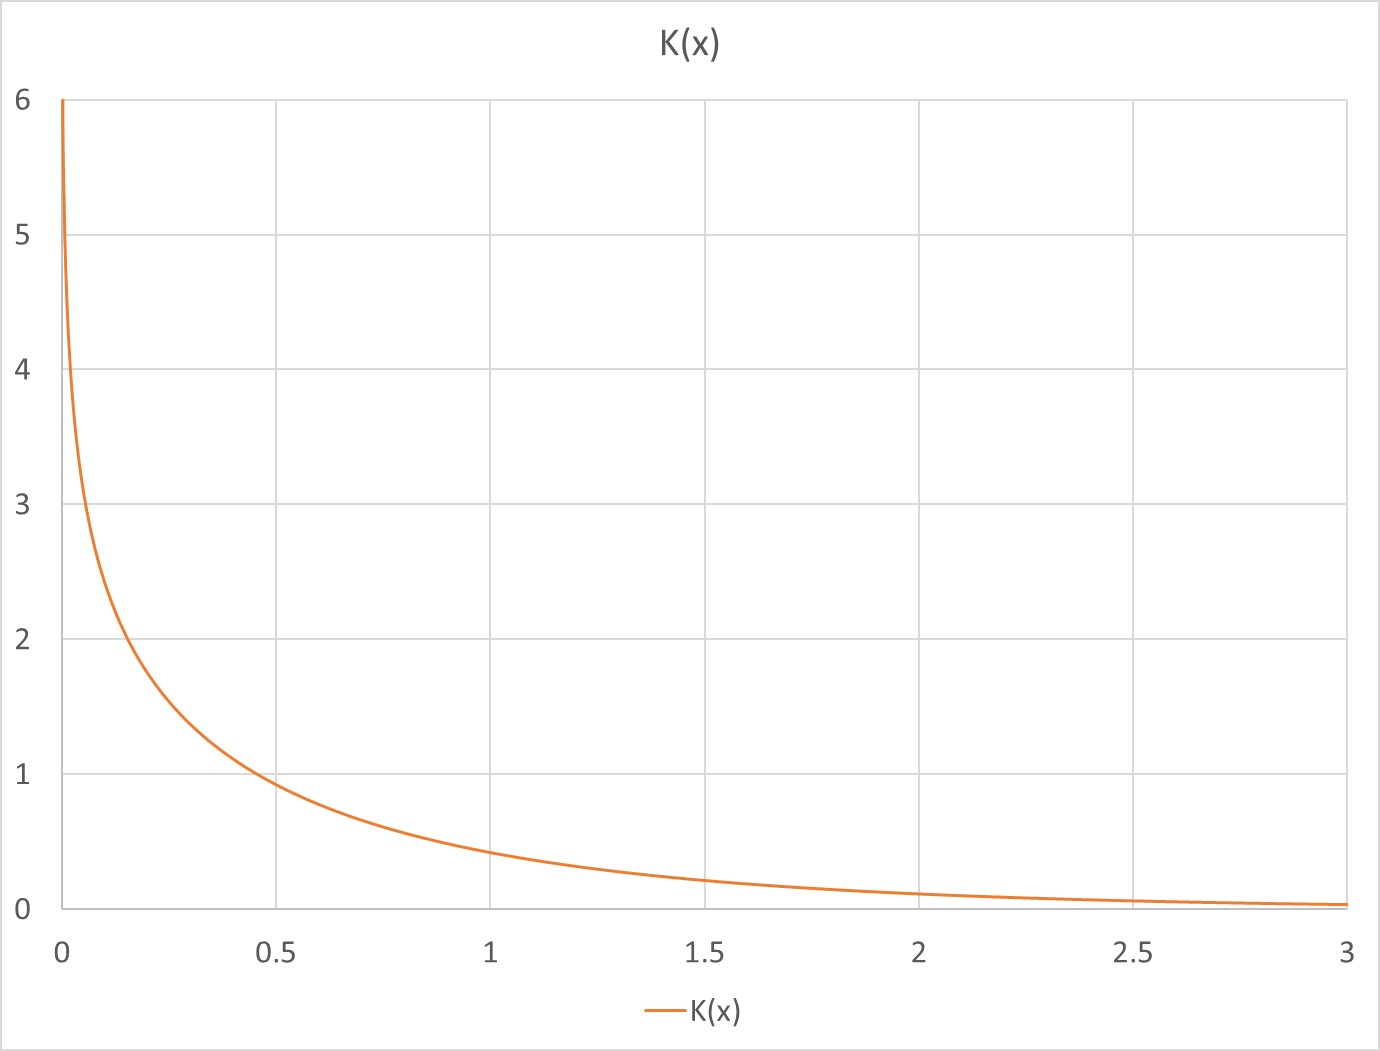
\includegraphics[width=.8\linewidth]{K_bessel.jpg}
\end{figure}
Based on the figure, it shows that $x\rightarrow 0$, then $K_0 = \infty$, hence, $C$ must be zero.
\bigbreak
Using boundary condition 2 and the formula taken from pg 146 of "Nuclear Reactor Physics" by E. E. Lewis:
\begin{align*}
    0 &= J^-\bigg(\frac{T}{2}\bigg) = \frac{\phi\bigg(\frac{T}{2}\bigg)}{4}+\frac{D}{2}\phi'\bigg(\frac{T}{2}\bigg) \\
    0 &= 0.25\bigg[AI_0\bigg(B\frac{T}{2}\bigg)+\frac{S_0}{\Sigma_a}\bigg]+\frac{D}{2}B\bigg[AI_1\bigg(B\frac{T}{2}\bigg)\bigg] \\
    0 &= A\bigg[I_0\bigg(B\frac{T}{2}\bigg)+2DBI_1\bigg(B\frac{T}{2}\bigg)\bigg]+\frac{S_0}{\Sigma_a} \\
    A &= -\frac{\frac{S_0}{\Sigma_a}}{I_0(B\frac{T}{2})+2DBI_1(B\frac{T}{2})}
\end{align*}
Thus the explicit equation for flux in the cylinder is:
\boxed{
\begin{equation*}
    \phi(r) = \frac{S_0}{\Sigma_a}\bigg[1-\frac{I_0(Br)}{I_0(B\frac{T}{2})+2DBI_1(B\frac{T}{2})}\bigg]
\end{equation*}
}
%###############################################################################
\newpage
\bigbreak
c) The approximate form of the diffusion equation for a spherical reactor is given below:
\bigbreak
\begin{equation*}
    \frac{1}{r^2}\frac{d}{dr}\bigg(r^2 \frac{d\phi(r)}{dr}\bigg) +B^2\phi(r) + \frac{S(r)}{D} = 0
\end{equation*}
\begin{figure}[h!]
                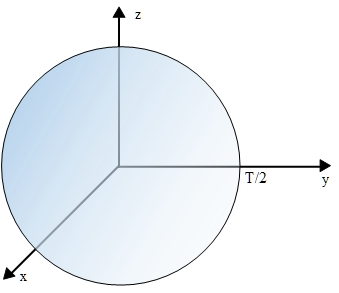
\includegraphics[width=.45\linewidth]{P1c.jpg}
\end{figure}
\bigbreak
The general solution form is shown below:
\bigbreak
\[   \phi(r) = \left\{
\begin{array}{ll}
      A\frac{e^{Br}}{r} + C\frac{e^{-Br}}{r}, &  B^2 < 0\\
      A\frac{\sin(Br)}{r} + C\frac{\cos(Br)}{r}, &  B^2 > 0\\
\end{array}
\right. \]
\bigbreak
The boundary conditions for this geometry are given below:
\begin{itemize}
    \item $\lim_{r \rightarrow 0}Jr4\pi r^2$ = 0
    \item $J^-$(T/2) = $J^+$(-T/2) = 0
    \item $\phi(0) \neq \infty$
    \item $\lim_{x\to\infty} \phi(x)$ = 0
\end{itemize}
Instead of using the above general solution for $B^2 < 0$, a general solution using $\sinh$ and $\cosh$ can be developed:
\begin{equation*}
    \phi(r) = \frac{A\sinh(Br)}{r}+\frac{C\cosh(Br)}{r}+\frac{S_0}{\Sigma_a}
\end{equation*}
Using boundary condition 1, and the equation $Jr = -D\phi'$:
\begin{align*}
    0 &= -4D\pi[A(B(0)\cosh(B(0))-\sinh(B(0)))+C(B(0)\sinh(B(0))-\cosh(B(0)))] \\
    0 &= -4D\pi C \\
    C &= 0
\end{align*}
Using boundary condition 2:
\begin{align*}
    0 &= J^-\bigg(\frac{T}{2}\bigg) = \frac{\phi\bigg(\frac{T}{2}\bigg)}{4} +\frac{D}{2}\phi'\bigg(\frac{T}{2}\bigg) \\
    0 &= 0.25\Bigg[\frac{A\sinh\bigg(B\frac{T}{2}\bigg)}{\frac{T}{2}}+\frac{S_0}{\Sigma_a}\Bigg] +\frac{D}{2}\Bigg[\frac{A\bigg[B\bigg(\frac{T}{2}\bigg)\cosh\bigg(B\bigg(\frac{T}{2}\bigg)\bigg)-\sinh\bigg(B\bigg(\frac{T}{2}\bigg)\bigg)\bigg]}{\bigg(\frac{T}{2}\bigg)^2}\Bigg] \\
    0 &= A\Bigg[\frac{\sinh\bigg(B\frac{T}{2}\bigg)}{\frac{T}{2}}+\frac{2D\bigg[B\bigg(\frac{T}{2}\bigg)\cosh\bigg(B\bigg(\frac{T}{2}\bigg)\bigg)-\sinh\bigg(B\bigg(\frac{T}{2}\bigg)\bigg)\bigg]}{\bigg(\frac{T}{2}\bigg)^2}\Bigg]+\frac{S_0}{\Sigma_a} \\
    A &= -\frac{\frac{S_0}{\Sigma_a}}{\frac{\sinh\bigg(B\frac{T}{2}\bigg)}{\frac{T}{2}}+\frac{2D\bigg[B\bigg(\frac{T}{2}\bigg)\cosh\bigg(B\bigg(\frac{T}{2}\bigg)\bigg)-\sinh\bigg(B\bigg(\frac{T}{2}\bigg)\bigg)\bigg]}{\bigg(\frac{T}{2}\bigg)^2}}
\end{align*}
Thus the explicit equation for flux in the sphere is:
\bigbreak
\boxed{
\begin{equation*}
    \phi(r) = \frac{S_0}{\Sigma_a}\Bigg[1-\frac{\sinh(Br)}{r}\frac{1}{\bigg(\frac{\sinh(B\frac{T}{2})}{\frac{T}{2}}+\frac{2D[B(\frac{T}{2})\cosh(B(\frac{T}{2}))-\sinh(B(\frac{T}{2}))]}{(\frac{T}{2})^2}\bigg)}\Bigg]
\end{equation*}
}
%###############################################################################
\newpage
\bigbreak
d) The approximate form of the diffusion equation for this system:
\bigbreak
\begin{equation*}
    \frac{d^2}{dx^2}\phi(x) + B^2\phi(x) = S(x)
\end{equation*}
 
\begin{figure}[h!]
                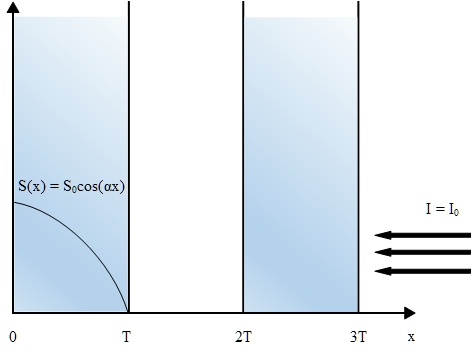
\includegraphics[width=.45\linewidth]{P1d.jpg}
\end{figure}
\bigbreak
The general solution form is shown below:
\bigbreak
\[   \phi(x) = \left\{
\begin{array}{ll}
      Ae^{-Bx} + Ce^{Bx} &  \\
      A'\sinh(Bx) + C'\cosh(Bx) &  \\
\end{array}
\right. , \quad B^2 < 0\]
\bigbreak
\[   \phi(x) = \left\{
\begin{array}{ll}
      Ae^{-iBx} + Ce^{iBx} &  \\
      A'\sin(Bx) + C'\cos(Bx) &  \\
\end{array}
\right. , \quad B^2 > 0\]
\bigbreak
The boundary conditions for this geometry are given below:
\begin{itemize}
    \item $J^+$(T) = $J^+$(2T)
    \item $J^-$(T) = $J^-$(2T)
    \item $\lim_{x \to \infty} \phi(x)$ = 0
\end{itemize}
\bigbreak
%%%%%%%%%%%%%%%%%%%%%%%%%%%%%%%%%%%%%%%%%%%%%%%%%%%%%%%%%%%%%%%%%%%%%%%%%%%%%%%%%%%%%%%%%%%%%%%%%%%%%%%%%%%%%%%%%%%%%%%%%%%
\newpage
\textbf{Problem 2:} Write a computer program to calculate the steady-state flux density distribution in a homogeneous infinite slab, sphere, and infinite cylinder each of which may contain an arbitrarily distributed volumetric source of neutrons. Assume vacuum boundary conditions.
\bigbreak
(a) Derive the first-order finite-difference form of the appropriate one-speed diffusion equation. Assume equal mesh spacing.\newline
\bigbreak
(b) Write the resulting equations in matrix form \textbf{$A\phi$} = \textbf{$s$}.\newline
\bigbreak
(c) Derive the TDMA algorithm to solve this set of equations and write a subroutine to implement this algorithm.\newline
\bigbreak
(d) Write a program to solve the 1-D finitie-difference diffusion equations developed in part (a). Input should include: geometry type, system size, number of mesh points desired, parameters $\Sigma_a$ and $D$, and the source distribution $S(r_i)$.\newline
\bigbreak
%%%%%%%%%%%%%%%%%%%%%%%%%%%%%%%%%%%%%%%%%%%%%%%%%%%%%%%%%%%%%%%%%%%%%%%%%%%%%%%%%%%%%%%%%%%%%%%%%%%%%%%%%%%%%%%%%%%%%%%%%%%
\newpage
\textbf{Solution}
\bigbreak
a) Below, a diagram is provided to understand node spacing for a slab, cylinder and spherical 1-D geometry. For this purpose, $h_i$ and $h_{i+1}$ are equivalent and denoted as $d_i$.
\bigbreak
\begin{figure}[h!]
                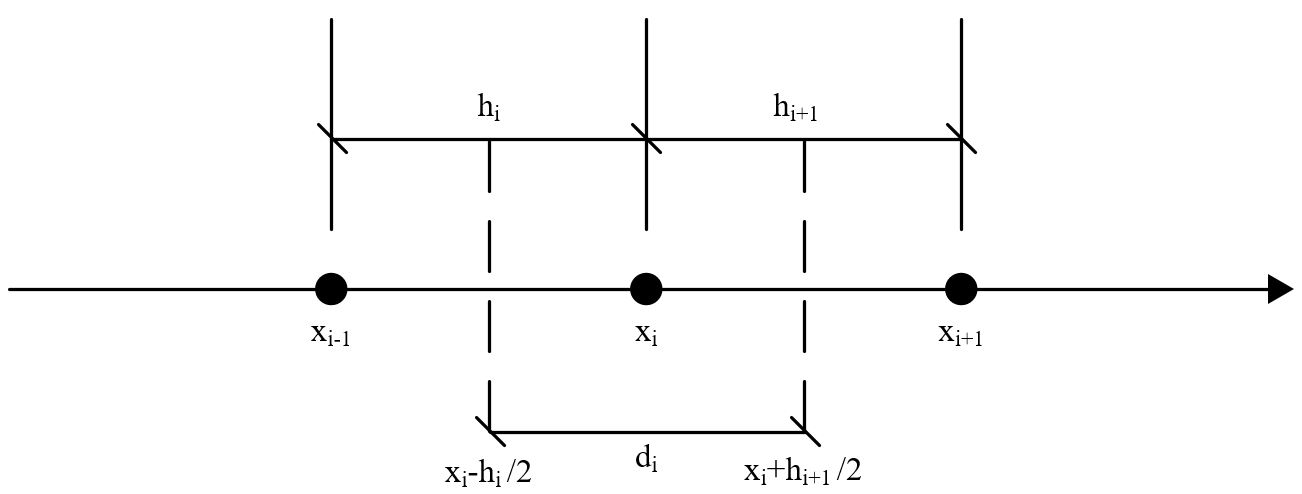
\includegraphics[width=.7\linewidth]{FD2.JPG}
\end{figure}
Using this pattern, nodes are spaced equidistant from each other spanning the thickness of the geometry. In the case of the cylindrical and spherical geometry, based on symmetry about the center, nodes are spaced from the center to the outer surface. Using the one-speed NDE for each geometry:
\begin{align*}
    S(x) &= -D\frac{d^2}{dx^2}\phi(x) + \Sigma_a\phi(x), \quad &(slab)  \\
    S(x) &= -D\frac{d^2}{dx^2}\phi(x) + \frac{1}{x}\frac{d}{dx}\phi(x) +\Sigma_a\phi(x), \quad &(cylinder) \\
    S(x) &= -D\frac{1}{x^2}\frac{d}{dx}\bigg(x^2 \frac{d\phi(x)}{dx}\bigg) +\Sigma_a\phi(x), \quad &(sphere)
\end{align*}
Which can be implicitly written as:
\begin{equation*}
    x^c S(x) = -D\frac{d}{dx}\bigg(x^c\frac{d\phi(x)}{dx}\bigg)+x^c\Sigma_a\phi(x)
\end{equation*}
Using this implicit form where c = 0 (slab), c=1 (cylinder), c=2 (sphere), the 1-D Finite Difference forms can be determined. Each term is integrated for domain $d_i$.
\begin{align*}
    \int_{x_i-d/2}^{x_i+d/2}dxS(x)x^c  &= -D\int_{x_i-d/2}^{x_i+d/2}dx\bigg[\frac{d}{dx}\bigg(x^c\frac{d\phi(x)}{dx}\bigg)\bigg]+\int_{x_i-d/2}^{x_i+d/2}dx \Sigma_a\phi(x)x^c\\
    S(x)x^cd &= -Dx^c\frac{d\phi(x)}{dx}\Biggr|_{x_i-d/2}^{x_i+d/2}+\Sigma_a\phi(x)x^cd\\
    S(x)x^cd &= -D(x_i+d/2)^c\bigg[\frac{\phi_{i+1}-\phi_i}{d}\bigg]+D(x_i-d/2)^c\bigg[\frac{\phi_i-\phi_{i-1}}{d}\bigg]+\Sigma_a\phi(x)x^cd
\end{align*}
\bigbreak
Thus the final solution is:
\boxed{S(x)x^cd =-D(x_i+d/2)^c\bigg[\frac{\phi_{i+1}-\phi_i}{d}\bigg]+D(x_i-d/2)^c\bigg[\frac{\phi_i-\phi_{i-1}}{d}\bigg]+\Sigma_a\phi(x)x^cd}
 
\newpage
b) Coefficients for each flux term can be solved using the equation, $A\phi = s$. Dividing each term, from the previous part, by $x^cd$ gives the matrix form:
\bigbreak
\boxed{a_{i,i-1}\phi_{i-1}+a_{i,i}\phi_{i}+a_{i,i+1}\phi_{i+1}=S_i}
\bigbreak
where $a_{i,i-1}$, $a_{i,i}$, and $a_{i,i+1}$ are defined as:
\begin{align*}
    a_{i,i-1} &= -\frac{D}{d^2}\bigg(1-\frac{1}{2i}\bigg)^c \\
    a_{i,i} &= \Sigma_a+\frac{D}{d^2}\bigg[\bigg(1-\frac{1}{2i}\bigg)^c+ \bigg(1+\frac{1}{2i}\bigg)^c\bigg] \\
    a_{i,i+1} &= -\frac{D}{d^2}\bigg(1+\frac{1}{2i}\bigg)^c
\end{align*}
\bigbreak
c) The matrix format is shown below and provided is the derivation of the TDMA algorithm:
\begin{figure}[h!]
                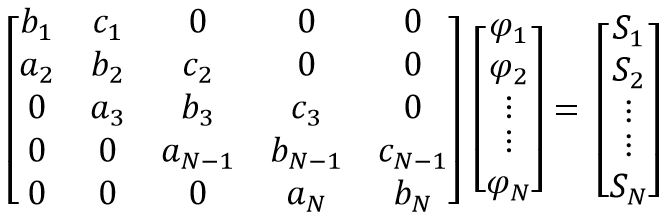
\includegraphics[width=.5\linewidth]{TDMA.JPG}
\end{figure}
\bigbreak
First we do forward elimination, going from row 2 to N:
\begin{align*}
    m &= \frac{a_i}{b_{i-1}} \\
    b_i &= b_i - mc_{i-1} \\
    d_i &= d_i - md_{i-1}
\end{align*}
This algorithm is characterized in the following product series are found:
\begin{align*}
    b_i &= b_i - \prod_{i = 2}^{N} (a_i)^{-i^{(i-1)}} (b_{i-1})^{-i^{(i)}} (c_{i-1})^{-i^{(i-1)}}, \quad i>2 \\
    S_i &= S_i - \prod_{i = 2}^{N} (a_i)^{-i^{(i-1)}} (b_{i-1})^{-i^{(i)}} (S_{i-1})^{-i^{(i-1)}}, \quad i>2
\end{align*}
Then backward substitution is applied for rows n-1 to 1:
\begin{align*}
    \phi_i &= \frac{S_i}{b_i} \\
    \phi_i &= \frac{S_i-c_i\phi_{i+1}}{b_i}
\end{align*}
This algorithm is characterized in the following product series are found:
\begin{align*}
    b_i &= b_i - \prod_{i = 2}^{N} (a_i)^{-i^{(i-1)}} (b_{i-1})^{-i^{(i)}} (c_{i-1})^{-i^{(i-1)}}, \quad i>2 \\
    S_i &= S_i - \prod_{i = 2}^{N} (a_i)^{-i^{(i-1)}} (b_{i-1})^{-i^{(i)}} (S_{i-1})^{-i^{(i-1)}}, \quad i>2
\end{align*}
 
%%%%%%%%%%%%%%%%%%%%%%%%%%%%%%%%%%%%%%%%%%%%%%%%%%%%%%%%%%%%%%%%%%%%%%%%%%%%%%%%%%%%%%%%%%%%%%%%%%%%%%%%%%%%%%%%%%%%%%%%%%%
\newpage
\textbf{Problem 3:} Use your program to solve the first three problems of question 1. Data to be used are: $D$ = 0.600 cm, $\Sigma_a$ = 0.005 $cm^{-1}$, $T$ = 45 cm, and $S_0$ = $10^8$ neutrons cm${}^{-2}$ s${}^{-1}$. Plot both the numerical solution and the analytical flux profile for each problem. Also investigate the effect of mesh size on the accuracy of the solutions.
\bigbreak
%%%%%%%%%%%%%%%%%%%%%%%%%%%%%%%%%%%%%%%%%%%%%%%%%%%%%%%%%%%%%%%%%%%%%%%%%%%%%%%%%%%%%%%%%%%%%%%%%%%%%%%%%%%%%%%%%%%%%%%%%%%
\newpage
\textbf{Solution}
 
\bigbreak
%%%%%%%%%%%%%%%%%%%%%%%%%%%%%%%%%%%%%%%%%%%%%%%%%%%%%%%%%%%%%%%%%%%%%%%%%%%%%%%%%%%%%%%%%%%%%%%%%%%%%%%%%%%%%%%%%%%%%%%%%%%
\end{document}
